% Case-A zero-lever response by commanded condition. The conditions are
% categorical, so they are labelled by the command itself rather than by the
% measured initial angle, which stays in Table~\ref{tab:results_case_a}.
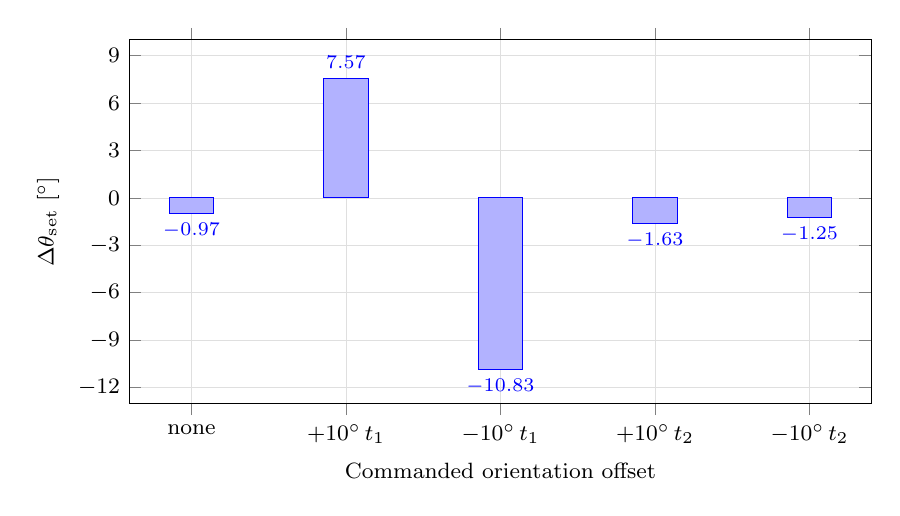
\begin{tikzpicture}
\begin{axis}[
    width=11.0cm, height=6.2cm,
    ybar,
    bar width=16pt,
    xtick=data,
    symbolic x coords={none, p10t1, m10t1, p10t2, m10t2},
    xticklabels={none, \(+10^\circ\,t_1\), \(-10^\circ\,t_1\),
                 \(+10^\circ\,t_2\), \(-10^\circ\,t_2\)},
    ymin=-13, ymax=10,
    ytick={-12,-9,-6,-3,0,3,6,9},
    grid=major,
    grid style={gray!25, very thin},
    tick label style={font=\footnotesize},
    label style={font=\footnotesize},
    xlabel={Commanded orientation offset},
    ylabel={\(\Delta\theta_{\mathrm{set}}\) [\(^\circ\)]},
    every axis plot/.append style={draw=black, fill=blue!20!white},
    nodes near coords,
    nodes near coords style={font=\scriptsize, /pgf/number format/fixed,
                             /pgf/number format/precision=2},
  ]
\addplot coordinates {
  (none,-0.97) (p10t1,7.57) (m10t1,-10.83) (p10t2,-1.63) (m10t2,-1.25)};
\end{axis}
\end{tikzpicture}
